%\documentclass[a4paper]{fhnwreport} %Legt grundlegende Formatierungen wie Schriftarten, Ort Seitenzahlen etc. fest.
%
%\graphicspath{{./graphics/}}%Change according to graphics folder!
%
%\begin{document}

\section{Hardware}

Der Hardware Teil ist in zwei Bereiche unterteilt: Sensorplatine und Kontrollplatine. Die Sensorplatine hat die Aufgabe die Spannungswerte der Solarzelle zu messen und diese über die Powerline an den Kontrollprint zu übermitteln.
Der Kontrollprint vergleicht diese Messwerte mit den Sollwerten einer funktionierenden Solarzelle und entscheidet dann, ob diese noch funtkionsfähig ist. Falls dem nicht so ist, wird ein Relaiskontakt geschlossen und es wird auf dem Display angezeigt, welches Panel defekt ist. 
Die Kommunikation zwischen diesen beiden Platinen darf keine zusätzlichen Kabel benötigen, dies bedingt, dass die übermittelten Werte auf die Powerline moduliert werden müssen. Dieser Aufbau ist im Hardwarekonzept (Abbildung \ref{fig::Hardwarekonzept}) zu sehen.
%Der Sensorprint wird über das Solarpanel gespiesen. Es ist deshalb darauf zu achten, das die Leistung nicht mehr als 100mW beträgt.

%Die Kommunikation über die Powerline (PLC) wird mittels eines Powerline Transceivers/Receivers realisiert.
\begin{figure}[h]
\centering
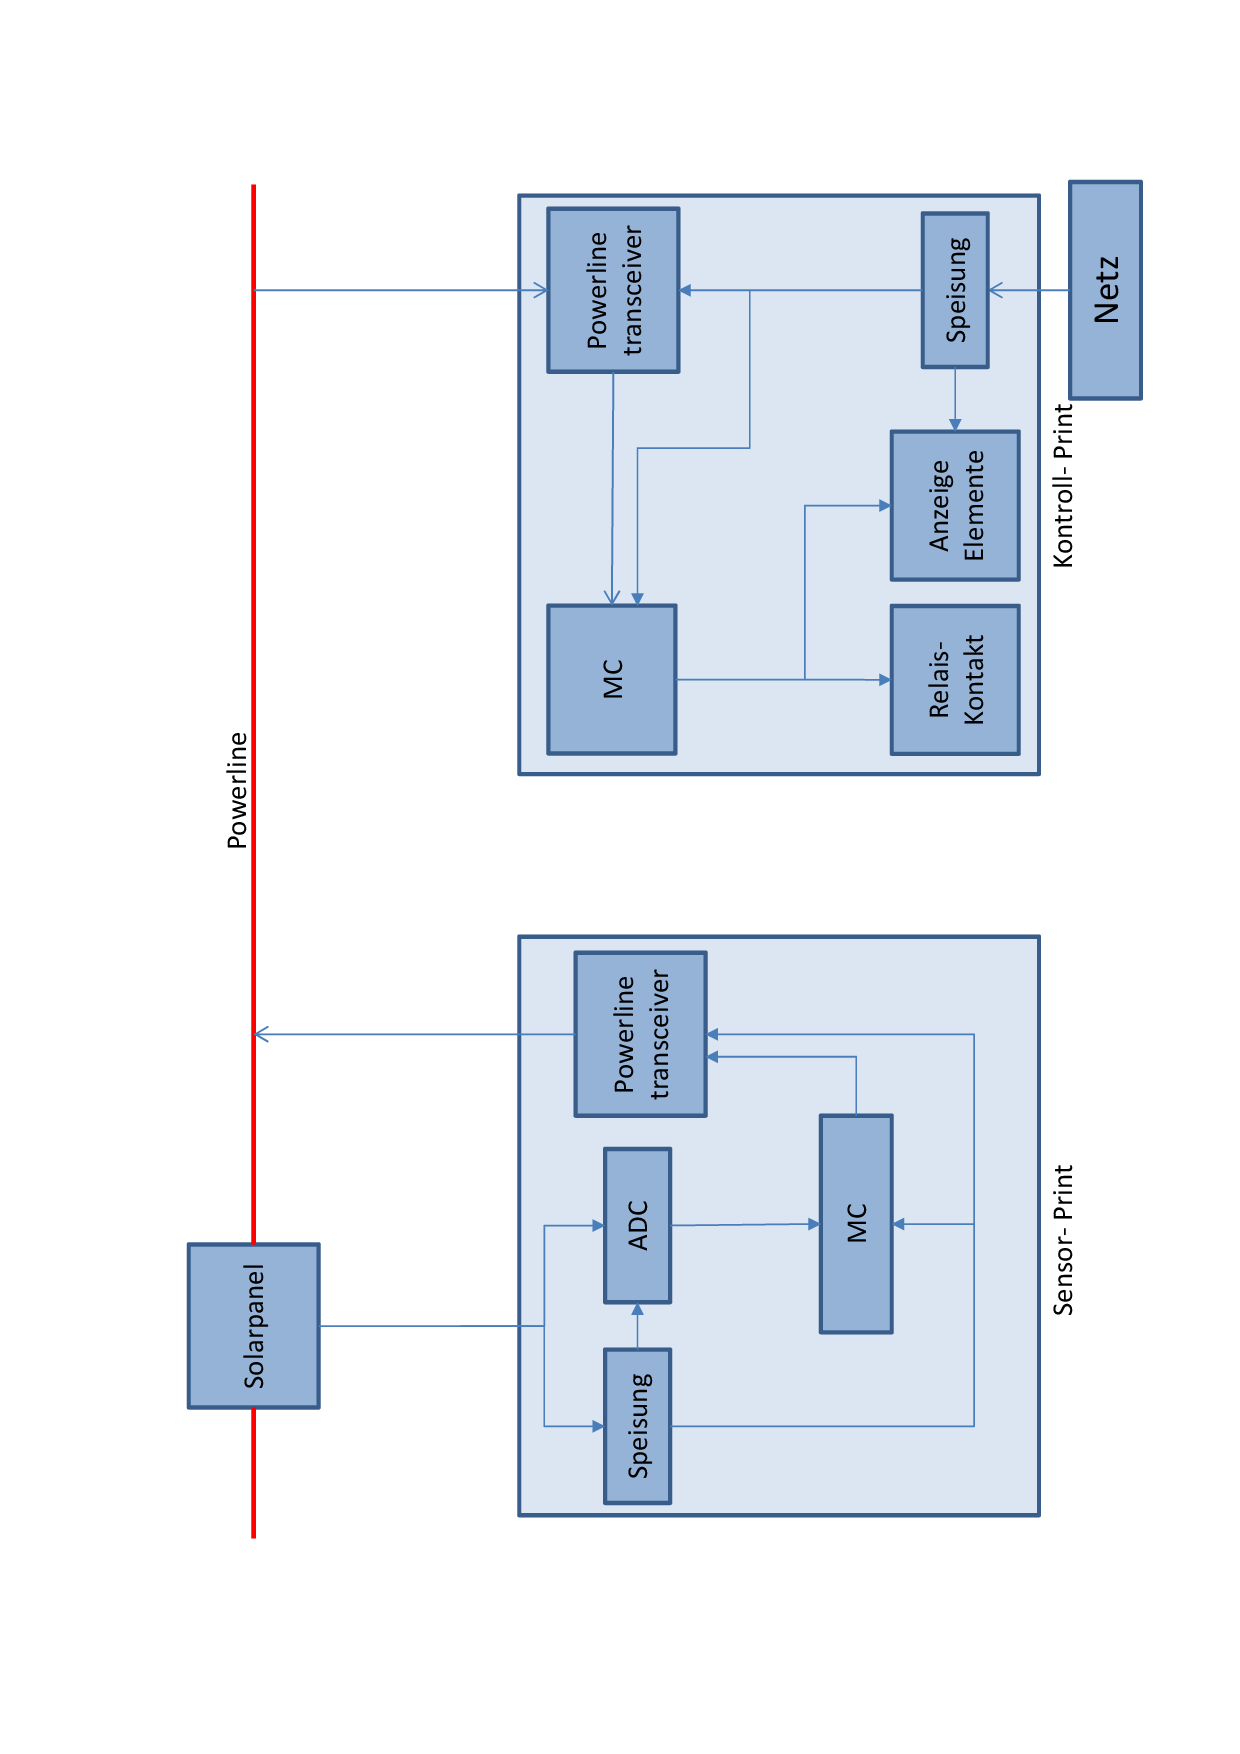
\includegraphics[angle = -90, width=1.0\textwidth]{Hardware_Konzept.png}%
\caption{Hardwarekonzept}
\label{fig::Hardwarekonzept}%
\end{figure}

\subsection{Sensorplatine}


Die Sensorplatine wird auf der Rückseite des Solarpanels angebracht. Es wird vom Solarpanel selbst gespiesen, weshalb auf möglichst kleine Leistungen geachtet werden muss. Die momentanen Spannungswerte des Solarpanels werden über einen AD-Wandler eingelesen und mit einem Mikrocontroller für den Powerline Transceiver entsprechend kodiert. Die kodierten Spannungswerte werden dann mittels eines Powerline Transceivers auf die Powerline eingekoppelt und so auf die Kontrollplatine übertragen. Für die Identifikation des Solarpanels kann auf der Platine mittels DIL-Schaltern eine binäre ID eingestellt werden.

\newpage
\subsubsection{Powerline Transceiver}

Es wurde für einen Powerline Transceiver entschieden, da das Übertragungsprotokoll FSK (Frequency Shift Keying) schon gegeben ist und es aufgrund mangelnder Fachlichen Vorkenntnissen in einem zu grossen zeitlichen Aufwand resultieren würde, wenn diese Einkopplung in die Powerline selbst entwickelt werden würde. 
Dieser Transceiver hat die Aufgabe die vom Mikrocontroller kodierten Spannungswerte auf die Powerline zu übertragen.

\subsubsection{Spannungsmessung}

Die Spanungsmessung erfolgt über eine OP-Schaltung, welche de Spannungsbereich von 5-60V auf 0.42-5V hinabskaliert. Diese werden dann über einen AD-Wandler eingelesen und an den MC weitergegeben.

\subsubsection{AD Wandler}

Der AD Wandler soll mindestens 10 Bit Auflösung haben und die Werte seriell ausgeben können. Dieser empfängt die skalierten Spannungswerte und digitalisiert diese für den Mikrocontroller.

\subsubsection{Mikrocontroller}

Der Mikrocontroller verschlüsselt die eingelesenen Werte nach FSK und sendet diese an den Powerline Transceiver.

\subsection{Kontrollplatine}

Die Kontrollplatine empfängt die modulierten Signale welche von der Sensorplatine über die Powerline übertragen werden. Diese Platine wird am Ende der Solaranlage in der Kontrollstation montiert. Dort kann der Anwender oder der Prüfer dieser Anlage herausfinden, ob defekte Solarpanels vorhanden sind.

\subsubsection{Speisung}
Die Speisung der Kontrollplatine erfolgt über das Netz. Die Netzspannung wird über ein Netzgerät auf eine definiert DC Spannung transformiert. 
Da mehrere Bauteile noch nicht definiert sind, kann die genaue DC Spannung noch nicht bestimmt werden. Die Speisung speist den Mikrocontroller, den Powerline transceiver und die Anzeigeelemente.

\subsubsection{Powerline transceiver}
Es wird der selbe Powerline transceiver wie bei der Sensorplatine verwendet. Dieser hat die Aufgabe die Modulierten Signale über die Powerline zu empfangen und diese dann zu entmodulieren. Danach werden die verarbeiteten Signale an den Mikrocontroller übermittelt.

\subsubsection{Microkontroller}
Die Signale werden vom Mikrocontroller empfangen und abgespeichert. Wenn alle Signale abgespeichert sind, werden diese ausgewertet. Danach wird entschieden ob die einzelnen Panels funtionstüchtig oder defekt sind. Als Microkontroller wird der ATMega328 verwendet.

\subsubsection{Anzeige Elemente}
Als Anzeige Element wird ein Display verwendet. An diesem kann abgelesen werden, welche Panels defekt sind. Zudem sind 2 LEDs vorhanden(Grün: ok, Rot: defekt).

\subsubsection{Relais Kontakt}
Wenn die Sollspannung eines Panels nicht erreicht wird, steuert der Mikrocontroller einen Relaiskontakt an, an welchem externe Geräte galvanisch getrennt angeschlossen werden können.

%\end{document}
